\documentclass[11pt,a4paper]{article}

% ------------------------------------------------------------------
% Packages
% ------------------------------------------------------------------
\usepackage[T1]{fontenc}
\usepackage[utf8]{inputenc}
\usepackage{lmodern}
\usepackage[margin=2.5cm]{geometry}
\usepackage{booktabs}
\usepackage{tabularx}
\usepackage{array}
\usepackage{xcolor}
\usepackage{listings}
\usepackage{tikz}
\usetikzlibrary{positioning,arrows.meta,fit,backgrounds}
\usepackage{enumitem}
\usepackage{hyperref}
\usepackage{caption}

\hypersetup{colorlinks=true, linkcolor=blue!50!black, urlcolor=blue!50!black}

\definecolor{codebg}{gray}{0.96}
\lstset{
  basicstyle=\ttfamily\small,
  backgroundcolor=\color{codebg},
  frame=single,
  rulecolor=\color{gray!40},
  breaklines=true,
  columns=fullflexible,
  keepspaces=true,
  showstringspaces=false,
  keywordstyle=\color{blue!60!black}\bfseries,
  commentstyle=\color{green!40!black},
}

\newcommand{\code}[1]{\texttt{#1}}
\newcolumntype{Y}{>{\raggedright\arraybackslash}X}

% ------------------------------------------------------------------
\title{Analysis of the Previous Group's FPGA Matrix-Multiplication Accelerator\\[4pt]
\large Setup, architecture review, bottlenecks and proposed improvements}
\author{Kai}
\date{\today}

\begin{document}
\setlength{\emergencystretch}{3em}
\maketitle

\begin{abstract}
\noindent
This report documents my analysis of the matrix-multiplication accelerator that the previous project group built for the Zynq UltraScale+ (ZCU102, \code{xczu9eg-ffvb1156-2-e}) using Vivado/Vitis 2025.1.1. I first describe what was needed to get their project to open and build on my machine. I then walk through the hardware and software architecture, estimate where the clock cycles go, and list the inefficiencies and issues I found. Finally I propose a set of improvements and estimate their effect. My main finding is that the design is dominated by data movement: the actual $5\times5$ block multiplication takes about 5 cycles, while fetching its operands takes about 100, and loading the matrices from the processor takes longer still. I estimate that the full set of proposed changes could make the end-to-end run roughly 50--100$\times$ faster. All numbers in this report are estimates from reading the design; they have not yet been measured on hardware.
\end{abstract}

\tableofcontents
\newpage

% ==================================================================
\section{Introduction}
% ==================================================================
The goal of the project is to offload matrix multiplication from the ARM processing system (PS) to the programmable logic (PL) of the FPGA in order to accelerate it. The previous group implemented a design that multiplies two $50\times50$ matrices of 64-bit integers by splitting them into $5\times5$ blocks. They reported that transferring the matrices between the PS and the PL takes most of the time (roughly 800 of about 900 clock cycles in their measurement).

I received their files via Teams and analysed them with three questions in mind:
\begin{enumerate}[noitemsep]
  \item Can the project be opened and built without errors?
  \item How does the design work, and where does the time go?
  \item What can be changed to make it faster, and by how much?
\end{enumerate}

% ==================================================================
\section{Received files and project setup}
% ==================================================================

\subsection{Contents of the hand-over}
\begin{table}[h]
\centering
\begin{tabularx}{\textwidth}{@{}lY@{}}
\toprule
\textbf{File} & \textbf{Contents} \\
\midrule
\code{S7\_integration.zip} (1.27\,GB) & Complete Vivado project (\code{S7\_integration.xpr}), block design \code{accu\_to\_DDR}, several exported \code{.xsa} files. \\
\code{S7\_integration\_vit.zip} & Vitis Unified workspace: platform \code{interrupt\_rerun\_plat} and application \code{interrupt\_rerun\_test}. \\
\code{DDR\_INTERFACE\_100MHz.zip} & Packaged HLS IP \code{RAM\_INTERFACE}. \\
\code{ip\_repo\_accumulator.zip} & Packaged IP \code{MatMul5x5\_Acc} (accumulator). \\
\code{ip\_repo\_matrix\_multiplier.7z} & Packaged IP \code{MatMul5x5\_PAR\_IF} (5$\times$5 multiplier). \\
\code{Matrix\_Partition\_Update.zip} & Packaged IP \code{matrix\_partitioner\_B}. \\
\code{ip\_matrix\_partition.zip} & Older \code{matrix\_partitioner} (not used in the final design). \\
\code{DDR\_interface HLS source files} & HLS C++ source of \code{RAM\_INTERFACE}. \\
\code{README.MD} & Short notes: use \code{C:/PLD/s7\_integration}, comment out the interrupt, tools are 2025.1.1. \\
\bottomrule
\end{tabularx}
\caption{Files received from the previous group.}
\end{table}

\subsection{Problems encountered during setup}
\begin{enumerate}
  \item \textbf{Absolute paths.} The Vivado project and the Vitis workspace contain absolute paths (e.g.\ the platform points to \code{C:\textbackslash PLD\textbackslash S7\_integration\textbackslash interrupt\_rerun.xsa}). I therefore used \code{C:\textbackslash PLD} as my workspace, with the Vivado project in \code{C:\textbackslash PLD\textbackslash S7\_integration} and the Vitis workspace in \code{C:\textbackslash PLD\textbackslash S7\_integration\_vit}. With this layout the Vitis platform and application built without any changes.
  \item \textbf{Tool version.} I initially had Vivado 2025.1 installed instead of 2025.1.1. In 2025.1 every IP in the block design (including standard Xilinx IP such as the Zynq PS, SmartConnect and BRAM controllers) was reported as ``Newer software version'' and locked, and the only offered action was ``Remove IP''. Installing 2025.1.1 resolved this for 143 of the 145 IPs.
  \item \textbf{IP repositories.} The project expects IP repositories at \code{../ip\_repo} and \code{../Cezar\_repo} relative to the project. I placed the four custom IPs in \code{C:\textbackslash PLD\textbackslash ip\_repo} and created an empty \code{Cezar\_repo} placeholder.
  \item \textbf{Outdated IP in the hand-over.} Two IPs remain locked with ``IP revision change'': \code{RAM\_INTERFACE} (design uses Rev.~2114456298, zip contains the older Rev.~2114452861) and \code{matrix\_partitioner\_B} (design uses Rev.~3, zip contains Rev.~1). I confirmed this by comparing the zipped sources with the copies Vivado keeps in \code{S7\_integration.gen/.../ipshared} (e.g.\ the design's \code{RAM\_INTERFACE.vhd} is 178\,KB, the zipped one 40\,KB). Clicking ``Upgrade IP'' would therefore \emph{downgrade} the design to an older version. The newest versions are most likely in the previous group's \code{Cezar\_repo}, which was not handed over. Until then the block design can be viewed but not validated or regenerated. The already exported hardware (\code{interrupt\_rerun.xsa} and bitstream) is unaffected and is what the Vitis platform uses.
\end{enumerate}

\subsection{Software build}
After setup, both the platform and the application build successfully in Vitis 2025.1.1. The remaining warnings in the platform build come from AMD's generated FSBL/PMU firmware and are harmless. I fixed the two warnings in \code{helloworld.c} (declaration order of \code{static volatile} and an unused handler parameter).

% ==================================================================
\section{Architecture of the previous design}
% ==================================================================

\subsection{Overview}
Figure~\ref{fig:arch} shows the data path as I reconstructed it from the block design \code{accu\_to\_DDR}. All user logic runs on a 100\,MHz clock (\code{addn\_ui\_clkout1} of the PL DDR4 controller); the DDR4 controller itself runs at 300\,MHz.

\begin{figure}[h]
\centering
\resizebox{\textwidth}{!}{%
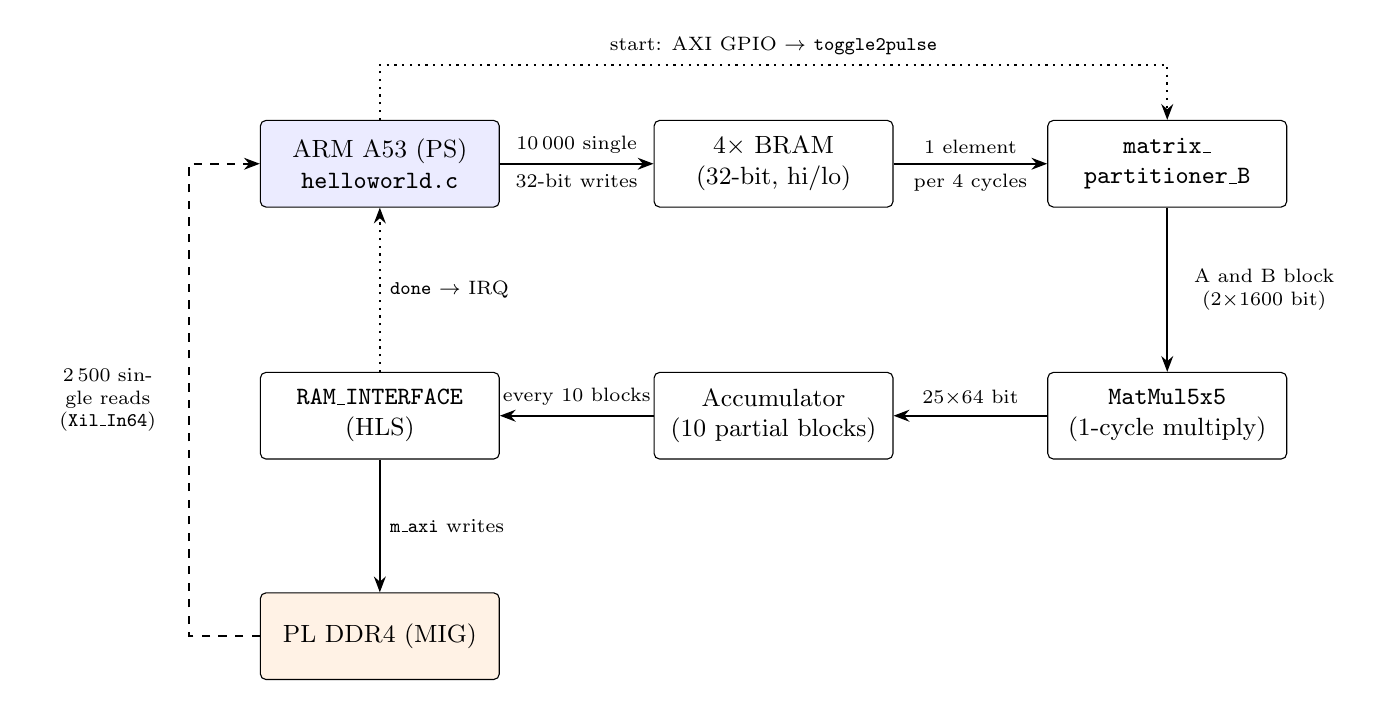
\begin{tikzpicture}[
  blk/.style={draw, rounded corners=2pt, align=center, minimum height=11mm, text width=28mm, font=\small, fill=white},
  arr/.style={-{Stealth[length=2mm]}, thick},
  lbl/.style={font=\scriptsize, align=center}
]
% row 1
\node[blk, fill=blue!8] (ps)   at (0,0)    {ARM A53 (PS)\\\code{helloworld.c}};
\node[blk]              (bram) at (5,0)  {4$\times$ BRAM\\(32-bit, hi/lo)};
\node[blk]              (part) at (10,0)   {\code{matrix\_}\\\code{partitioner\_B}};
% row 2
\node[blk]              (ram)  at (0,-3.2)   {\code{RAM\_INTERFACE}\\(HLS)};
\node[blk]              (acc)  at (5,-3.2) {Accumulator\\(10 partial blocks)};
\node[blk]              (mm)   at (10,-3.2)  {\code{MatMul5x5}\\(1-cycle multiply)};
% row 3
\node[blk, fill=orange!10] (ddr) at (0,-6) {PL DDR4 (MIG)};

\draw[arr] (ps) -- node[lbl, above]{10\,000 single}  node[lbl, below]{32-bit writes} (bram);
\draw[arr] (bram) -- node[lbl, above]{1 element} node[lbl, below]{per 4 cycles} (part);
\draw[arr] (part) -- node[lbl, right, text width=22mm]{A and B block\\(2$\times$1600 bit)} (mm);
\draw[arr] (mm) -- node[lbl, above]{25$\times$64 bit} (acc);
\draw[arr] (acc) -- node[lbl, above]{every 10 blocks} (ram);
\draw[arr] (ram) -- node[lbl, right]{\code{m\_axi} writes} (ddr);
\draw[arr, dotted] (ram) -- node[lbl, right]{\code{done} $\rightarrow$ IRQ} (ps);
\draw[arr, dashed] (ddr.west) -- ++(-0.9,0) |- node[lbl, pos=0.25, left, text width=18mm]{2\,500 single reads (\code{Xil\_In64})} (ps.west);
\draw[arr, dotted] (ps.north) -- ++(0,0.7) -| node[lbl, pos=0.25, above]{start: AXI GPIO $\rightarrow$ \code{toggle2pulse}} (part.north);
\end{tikzpicture}}
\caption{Data path of the previous design (reconstructed from the block design).}
\label{fig:arch}
\end{figure}

\subsection{Step by step}
\begin{enumerate}
  \item \textbf{Loading (PS).} \code{helloworld.c} writes matrices A and B ($50\times50$, 64-bit) into block RAM through AXI BRAM controllers (32-bit data width). Each 64-bit element is split into a high and a low 32-bit word stored in two separate BRAMs (\code{bram\_write\_64()}). This results in $2 \times 2500 \times 2 = 10\,000$ individual AXI write transactions, each issued by the CPU.
  \item \textbf{Start.} The PS writes an AXI GPIO output; \code{toggle2pulse} (pulse width 105 cycles) converts the level change into a start pulse for the partitioner.
  \item \textbf{Partitioning.} \code{matrix\_partitioner\_B} iterates over all block triples $(i,j,p)$ with $p$ fastest ($10\times10\times10 = 1000$ triples). For each triple it reads block $A_{ip}$ and block $B_{pj}$ element by element from the BRAMs, reassembles the 64-bit values, and outputs two 1600-bit vectors with a valid/ready handshake.
  \item \textbf{Block multiply.} \code{MatMul5x5\_PAR\_IF} wraps \code{MatMul5x5}, which computes $C = A \times B$ for the $5\times5$ blocks in a \emph{single} clock cycle (125 signed $64\times64$-bit multiplications and 128-bit additions). Only the lower 64 bits of each 128-bit result are passed on.
  \item \textbf{Accumulation.} \code{MatMul5x5\_Accumulator} (\code{NUM\_ACCUMULATIONS}~=~10) adds the 10 partial products $A_{ip}B_{pj}$ to form one output block $C_{ij}$.
  \item \textbf{Write-back.} The HLS block \code{RAM\_INTERFACE} (free-running, \code{ap\_ctrl\_none}) writes each finished $5\times5$ block to the PL DDR4 at \code{0x4\_0000\_0000} via an \code{m\_axi} port, and raises \code{done} after all 100 output blocks.
  \item \textbf{Completion and check.} \code{done} is connected to \code{pl\_ps\_irq0} and to a GPIO input. The software waits for the interrupt, computes the reference result on the CPU, and compares it with the result it reads back from PL DDR4 using 2\,500 single 64-bit reads.
\end{enumerate}

\subsection{Resource usage and timing}
From the implementation reports of their last build:

\begin{table}[h]
\centering
\begin{tabular}{@{}lrrr@{}}
\toprule
\textbf{Resource} & \textbf{Used} & \textbf{Available} & \textbf{Utilisation} \\
\midrule
CLB LUTs        & 50\,779 & 274\,080 & 18.5\,\% \\
CLB registers   & 80\,263 & 548\,160 & 14.6\,\% \\
Block RAM tiles & 244     & 912      & 26.8\,\% \\
DSP slices      & 1\,257  & 2\,520   & 49.9\,\% \\
\bottomrule
\end{tabular}
\caption{Utilisation after placement (previous group's build).}
\end{table}

All timing constraints are met. The 100\,MHz user clock has a worst negative slack of $+1.40$\,ns, i.e.\ the critical path is about 8.6\,ns. Half of the chip's DSP slices are used by the single-cycle $5\times5$ multiplier.

% ==================================================================
\section{Cycle budget}
% ==================================================================
I estimated the cycle counts by reading the RTL state machines (Table~\ref{tab:cycles}).

\begin{itemize}
  \item The partitioner cycles through \code{ISSUE\_ADDR} $\rightarrow$ \code{WAIT1} $\rightarrow$ \code{WAIT2} $\rightarrow$ \code{CAPTURE} for every element, i.e.\ 4 cycles per element. A block pair has 25 elements (A and B are read in parallel), so one block pair costs about $25 \times 4 = 100$ cycles plus the handshake.
  \item The multiplier needs about 5 cycles per block pair (accept, load, compute, done, output). Because the partitioner only presents a new block pair every $\sim$100 cycles, the multiplier is idle about 95\,\% of the time.
  \item \code{RAM\_INTERFACE} writes one output block every 10 block pairs ($\sim$1000 cycles), so it is not on the critical path.
\end{itemize}

\begin{table}[h]
\centering
\begin{tabular}{@{}lrr@{}}
\toprule
\textbf{Stage} & \textbf{Estimate} & \textbf{Time} \\
\midrule
Partitioner fetch, per block pair & $\sim$100 cycles & 1\,\textmu s \\
Block multiply, per block pair & $\sim$5 cycles & 50\,ns \\
Full PL run (1\,000 block pairs) & $\sim$102\,000 cycles & $\sim$1.0\,ms \\
PS loading (10\,000 AXI writes) & -- & $\sim$1--2\,ms (est.) \\
PS read-back (2\,500 uncached reads) & -- & $\sim$0.5--1\,ms (est.) \\
\midrule
\textbf{End-to-end} & & $\sim$\textbf{2.5--4\,ms} \\
\bottomrule
\end{tabular}
\caption{Estimated time budget of the current design at 100\,MHz. PS-side times depend on the (unmeasured) latency of a single PS$\rightarrow$PL transaction.}
\label{tab:cycles}
\end{table}

This supports the previous group's observation that data movement, not computation, dominates the run time. It holds both on the PS--PL boundary and inside the PL.

% ==================================================================
\section{Findings: inefficiencies and issues}
% ==================================================================
I list the findings roughly in order of their impact on performance.

\subsection{Data movement}
\begin{enumerate}[label=\textbf{F\arabic*}]
  \item \textbf{CPU-driven single-word loading.} Every element is written by the CPU as two separate 32-bit AXI transactions (10\,000 in total), with no bursts and no DMA. Each transaction crosses the PS--PL interconnect individually. This is almost certainly the largest cost in the system.
  \item \textbf{Unoptimised software build.} The application is compiled with \code{-O0 -g3} (visible in the build log), which makes the CPU loading loop considerably slower than necessary.
  \item \textbf{Unnecessary wait states in the partitioner.} The BRAMs have a read latency of 1 cycle (no output registers), and the address multipliers (\code{mult\_gen}, constant $\times4$) have 0 pipeline stages. The \code{WAIT1} and \code{WAIT2} states therefore serve no purpose; a new address could be issued every cycle.
  \item \textbf{One element per cycle at best.} Each matrix has only one read port in use, so even without wait states a block needs at least 25 cycles. The 64-bit values are also split over two 32-bit BRAMs, which doubles the number of memories and CPU writes.
  \item \textbf{No data reuse.} Every A block is read 10 times and every B block 10 times: 50\,000 element reads for 5\,000 unique elements.
  \item \textbf{Result path through PL DDR4.} Results are written to a separate PL DDR4 through a MIG controller (an extra 300\,MHz clock domain, clock-domain crossings and significant logic) and then read back by the CPU with 2\,500 uncached single reads over the HPM port. \code{RAM\_INTERFACE} writes each $5\times5$ block with strided addresses, so it can only form short bursts.
\end{enumerate}

\subsection{Compute}
\begin{enumerate}[label=\textbf{F\arabic*},resume]
  \item \textbf{Oversized, unpipelined multiplier.} All 125 $64\times64$-bit multiplications and their additions happen in one combinational cycle. This uses 1\,257 DSPs and prevents raising the clock above 100\,MHz. Meanwhile the unit is idle about 95\,\% of the time (F3--F5).
  \item \textbf{Word width larger than needed.} The test data are at most $2\,500^2 \times 50 \approx 3\times10^8$, which fits in 32 bits, and the inputs themselves fit in 16 bits. The upper 64 bits of each 128-bit product are discarded anyway.
  \item \textbf{Signed/unsigned mismatch.} \code{MatMul5x5} interprets the data as \code{signed}, while the software and the accumulator treat them as unsigned (\code{uint64\_t}, \code{unsigned}). This is harmless for the small positive test values but gives wrong results for large or negative inputs.
\end{enumerate}

\subsection{Robustness and measurement}
\begin{enumerate}[label=\textbf{F\arabic*},resume]
  \item \textbf{Interrupt never enabled.} In \code{helloworld.c} the GIC is configured and the handler connected, but \code{Xil\_ExceptionInit()}, \code{Xil\_ExceptionRegisterHandler()} and \code{Xil\_ExceptionEnable()} are never called, and no trigger type is set. The CPU therefore never takes the interrupt and the program hangs at ``Waiting for done signal''. This matches the README's remark that the interrupt never worked. I have added these calls (the original is kept in \code{backup/helloworld\_original.c}); the fix still has to be verified on the board.
  \item \textbf{Fragile handshakes.} \code{RAM\_INTERFACE} is free-running (\code{ap\_ctrl\_none}) and uses plain wires (\code{ap\_none}) for \code{valid}, \code{ready} and \code{done}, with its state kept in \code{static} variables. This is not a proper valid/ready protocol and can misbehave if \code{valid} is seen for more than one iteration. AXI-Stream interfaces (\code{hls::stream}) would make this well defined.
  \item \textbf{Debug logic left in.} Two System ILAs probe very wide buses (up to 1\,600 bits). They take block RAM and routing resources and make timing closure harder.
  \item \textbf{Inflated load measurement.} The ``BRAM load time'' also includes filling the CPU's own reference copies of the matrices (\code{test\_MatrixA/B}), so it overstates the pure transfer time.
  \item \textbf{Hand-over incomplete.} The previous group did not include the newest versions of two IPs, namely \code{RAM\_INTERFACE} and \code{matrix\_partitioner\_B}, nor the \code{Cezar\_repo} folder, so the block design cannot currently be regenerated (Section~2.2).
\end{enumerate}

% ==================================================================
\section{Proposed improvements}
% ==================================================================

\subsection{Quick wins (software only)}
\begin{itemize}
  \item Build the application with \code{-O2}.
  \item Measure the pure BRAM loading separately from filling the reference arrays.
  \item Time the CPU's own reference multiplication, which the program already performs. This gives the baseline the accelerator has to beat.
\end{itemize}

\subsection{Small hardware changes}
\begin{itemize}
  \item Remove \code{WAIT1}/\code{WAIT2} and pipeline the address generation so the partitioner reads one element per cycle ($\sim$4$\times$ faster PL side).
  \item Replace each pair of 32-bit BRAMs with one 64-bit BRAM (64-bit BRAM controller on the 128-bit HPM0 port). This halves the number of CPU writes and removes the \code{mult\_gen} address multipliers (a constant $\times4$ is just a shift).
  \item Remove the ILAs in performance builds.
\end{itemize}

\subsection{Larger architectural changes}
\begin{itemize}
  \item \textbf{Let the PL move the data (largest gain).} Add a burst-capable master in the PL (an HLS block with \code{m\_axi} ports, or an AXI DMA) on \code{S\_AXI\_HP0\_FPD}, reading A and B directly from PS DDR and writing C back to PS DDR. The CPU only flushes/invalidates the caches and starts the transfer. At 128 bits per beat, the 40\,KB of input needs about 2\,500 beats instead of 10\,000 CPU transactions. This also makes the PL DDR4 and its MIG controller unnecessary.
  \item \textbf{Banked memory.} Distribute each matrix over 5 BRAM banks (interleaved by column) so that a full row of a $5\times5$ block is read in one cycle ($\sim$5 cycles per block instead of 25--100).
  \item \textbf{Data reuse.} Keep a row of A blocks on chip while iterating over the B blocks, or move to a systolic-array organisation, so that each element is fetched from memory once.
  \item \textbf{Narrower, pipelined compute.} Use 32-bit (or 16-bit) inputs if the application allows it and pipeline the multiply/add tree. This reduces DSP usage drastically and allows a 250--300\,MHz clock; the freed DSPs can be used for more parallel units.
  \item \textbf{Clean interfaces.} Use AXI-Stream between the blocks and an AXI-Lite control interface (\code{s\_axilite}) instead of GPIO plus \code{toggle2pulse}.
\end{itemize}

% ==================================================================
\section{Expected improvement}
% ==================================================================
Table~\ref{tab:gain} shows my estimate of the effect of each change on the part of the run it affects. Table~\ref{tab:total} compares the current and the fully improved design.

\begin{table}[h]
\centering
\begin{tabularx}{\textwidth}{@{}YYl@{}}
\toprule
\textbf{Change} & \textbf{Affects} & \textbf{Local speed-up} \\
\midrule
\code{-O2} build & PS loading loop & 1.5--3$\times$ \\
Remove \code{WAIT1}/\code{WAIT2} & PL fetch & $\sim$4$\times$ (102k $\rightarrow$ 26k cycles) \\
64-bit BRAM instead of 2$\times$32-bit & PS loading & $\sim$2$\times$ \\
Burst transfer (DMA / HLS \code{m\_axi}) & PS loading and read-back & \textbf{$\sim$50--100$\times$} \\
Banked BRAM + data reuse & PL fetch & $\sim$5$\times$ (26k $\rightarrow$ $\sim$5k cycles) \\
Narrow, pipelined MAC at 250\,MHz & PL compute & $\sim$2.5$\times$ (clock) \\
Remove PL DDR4 and ILAs & read-back, timing & enables the above \\
\bottomrule
\end{tabularx}
\caption{Estimated effect of each proposed change on the stage it affects.}
\label{tab:gain}
\end{table}

\begin{table}[h]
\centering
\begin{tabular}{@{}lcc@{}}
\toprule
\textbf{Stage} & \textbf{Current (est.)} & \textbf{After all changes (est.)} \\
\midrule
Loading A and B        & $\sim$1--2\,ms   & $\sim$15--20\,\textmu s \\
PL computation         & $\sim$1.0\,ms    & $\sim$5--20\,\textmu s \\
Result read-back       & $\sim$0.5--1\,ms & $\sim$5\,\textmu s \\
\midrule
\textbf{Total}         & \textbf{$\sim$2.5--4\,ms} & \textbf{$\sim$30--50\,\textmu s} \\
\bottomrule
\end{tabular}
\caption{Estimated end-to-end time before and after all proposed changes.}
\label{tab:total}
\end{table}

Overall I expect an end-to-end improvement of roughly \textbf{50--100$\times$}. About 70--80\,\% of that gain comes from a single change: letting the PL fetch and store the data in bursts instead of the CPU transferring every value. If time allows only one large change, it should be this one, combined with the cheap removal of the partitioner's wait states.

\subsection{Comparison with a CPU-only implementation}
An important caveat is the baseline. A straightforward $50\times50$ multiplication (125\,000 multiply-accumulates) on the Cortex-A53 compiled with \code{-O2} should take in the order of 0.1--0.2\,ms. By that estimate the \emph{current} accelerator is about 10--30$\times$ \emph{slower} than simply using the CPU, and the improved design would be about 3--5$\times$ faster than the CPU. For a matrix this small, fixed overheads (cache maintenance, starting the transfer, the interrupt) are a significant part of the total. The advantage of the accelerator grows with the matrix size, because computation scales with $n^3$ while data transfer scales with $n^2$.

% ==================================================================
\section{Next steps}
% ==================================================================
\begin{enumerate}
  \item Obtain the newest \code{RAM\_INTERFACE} and \code{matrix\_partitioner\_B} IP (\code{Cezar\_repo}) from the previous group, so the block design can be regenerated.
  \item On the board: verify the interrupt fix and run the existing design unchanged.
  \item Measure: (a) the latency of a single PS$\rightarrow$PL write, (b) the pure loading time, (c) the PL run time, and (d) the CPU-only multiplication time. These replace the estimates in this report with real numbers.
  \item Implement the quick wins and the partitioner wait-state removal, and measure again.
  \item Design the burst-based data path (PL master on \code{S\_AXI\_HP0\_FPD}) as the main architectural improvement.
\end{enumerate}

% ==================================================================
\section{Conclusion}
% ==================================================================
The previous group delivered a working hardware data path for blocked $50\times50$ matrix multiplication on the ZCU102, and I was able to set it up and build it with Vivado/Vitis 2025.1.1. My analysis shows that the design spends the vast majority of its time moving data: the CPU writes every value individually, the partitioner needs 4 cycles per element, blocks are re-read ten times, and results travel through a separate DDR4 and are read back one at a time. The compute unit itself is fast but oversized and idle about 95\,\% of the time. By letting the PL transfer data in bursts, removing the wait states, banking the memories and narrowing and pipelining the compute, I estimate the run time can be reduced from a few milliseconds to a few tens of microseconds. These estimates now need to be confirmed with measurements on the board.

\end{document}
